% Axes, element orientation and centres of pyfe3d.vabs.CrossSection
%
% Compile: pdflatex vabs_axes.tex
%          pdftocairo -svg vabs_axes.pdf vabs_axes.svg
%
% (a) Flared channel, centre line (1.4, 2) - (0, 1) - (0, -1) - (1.4, -2),
%     thickness 0.08, homogeneous and isotropic; the tension centre
%     (0.408, 0) and the shear centre (-0.453, 0), measured from the middle
%     of the web, are those computed by CrossSection.calc_stiffness. The
%     highlighted element of the upper flange has theta1 = atan(1/1.4).
% (b) Wall element seen from the tip of y3 = m3, ply angle theta3 = 30 deg.
\documentclass[border=2pt]{standalone}
\usepackage{tikz}
\usetikzlibrary{arrows.meta, calc}
\begin{document}
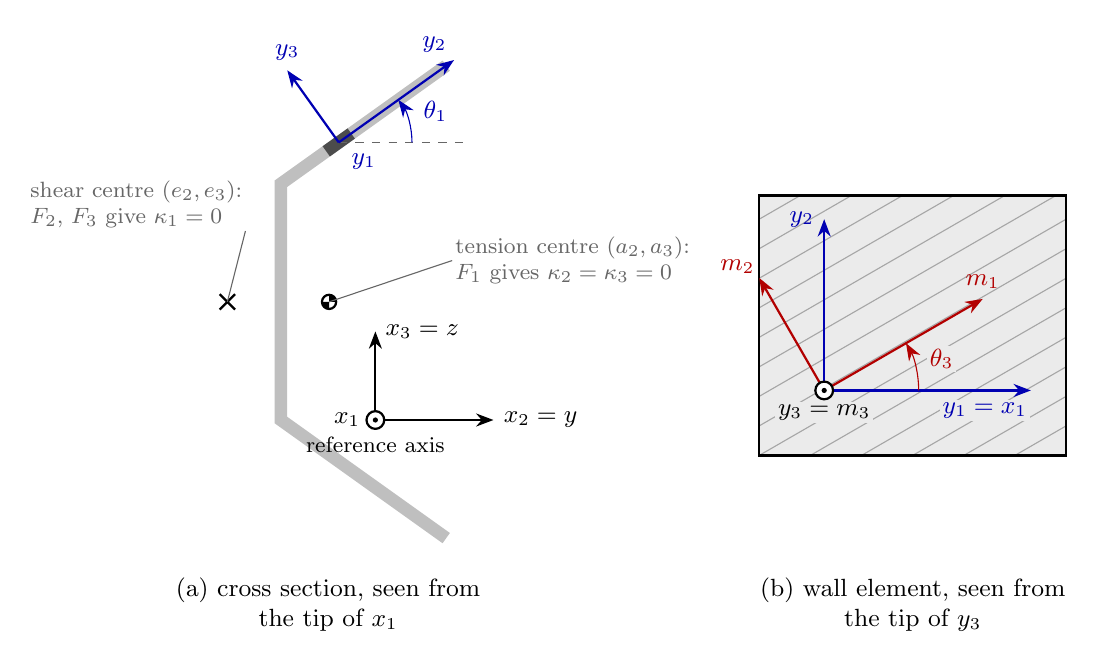
\begin{tikzpicture}[scale=1.5, >={Stealth[length=2.2mm]},
    ax/.style={->, thick},
    loc/.style={->, thick, blue!70!black},
    mat/.style={->, thick, red!70!black},
    lbl/.style={font=\small},
    note/.style={font=\footnotesize, align=left, inner sep=1pt}]

  % ------------------------------------------------------------- (a)
  \def\thone{35.54}
  % wall, centre line drawn with the wall thickness
  \draw[line width=1.6mm, black!25, line join=miter]
    (1.4, 2) -- (0, 1) -- (0, -1) -- (1.4, -2);
  % highlighted element of the upper flange
  \coordinate (P) at (0.49, 1.35);
  \fill[black!70, rotate around={\thone:(P)}]
    ($(P) + (-0.13, -0.053)$) rectangle ($(P) + (0.13, 0.053)$);
  % local axes y2, y3 of the element; y1 = x1 points to the viewer
  \draw[dashed, black!60] (P) -- ++(1.05, 0);
  \draw[loc] (P) -- ++(\thone:1.2) node[lbl, above left=-1pt] {$y_2$};
  \draw[loc] (P) -- ++(\thone + 90:0.75) node[lbl, above] {$y_3$};
  \draw[->, blue!70!black] ($(P) + (0.62, 0)$) arc[start angle=0,
    end angle=\thone, radius=0.62];
  \node[lbl, blue!70!black] at ($(P) + (\thone/2:0.86)$) {$\theta_1$};
  \node[lbl, blue!70!black, below right=-1pt] at ($(P) + (0.05, -0.04)$)
    {$y_1$};

  % reference axis: origin of x2, x3; x1 points to the viewer
  \coordinate (O) at (0.8, -1.0);
  \draw[ax] (O) -- ++(1.0, 0) node[lbl, right] {$x_2 = y$};
  \draw[ax] (O) -- ++(0, 0.75) node[lbl, right] {$x_3 = z$};
  \draw[thick, fill=white] (O) circle (0.075);
  \fill (O) circle (0.022);
  \node[lbl, left=2pt] at (O) {$x_1$};
  \node[note, below=5pt] at (O) {reference axis};

  % centres, measured from the reference axis
  \coordinate (T) at (0.408, 0);
  \coordinate (S) at (-0.453, 0);
  \draw[thick] (T) circle (0.06);
  \fill (T) -- ++(0.06, 0) arc[start angle=0, end angle=90, radius=0.06]
    -- cycle;
  \fill (T) -- ++(-0.06, 0) arc[start angle=180, end angle=270,
    radius=0.06] -- cycle;
  \draw[thick] ($(S) + (-0.065, -0.065)$) -- ($(S) + (0.065, 0.065)$)
    ($(S) + (-0.065, 0.065)$) -- ($(S) + (0.065, -0.065)$);
  \draw[black!60] (T) -- (1.45, 0.35)
    node[note, anchor=west] {tension centre $(a_2, a_3)$:\\
      $F_1$ gives $\kappa_2 = \kappa_3 = 0$};
  \draw[black!60] (S) -- (-0.3, 0.6)
    node[note, anchor=south east] {shear centre $(e_2, e_3)$:\\
      $F_2$, $F_3$ give $\kappa_1 = 0$};

  \node[font=\small, align=center, anchor=north] at (0.4, -2.25)
    {(a) cross section, seen from\\ the tip of $x_1$};

  % ------------------------------------------------------------- (b)
  \begin{scope}[shift={(4.05, -1.3)}]
    \def\ththree{30}
    \def\W{2.6}
    \def\H{2.2}
    \fill[black!8] (0, 0) rectangle (\W, \H);
    \begin{scope}
      \clip (0, 0) rectangle (\W, \H);
      \foreach \s in {-3.0, -2.75, ..., 3.0} {
        \draw[black!35] ($(0, \s)$) -- ++(\ththree:6);
      }
    \end{scope}
    \draw[thick] (0, 0) rectangle (\W, \H);
    \coordinate (Q) at (0.55, 0.55);
    \draw[loc] (Q) -- ++(1.75, 0) node[lbl, anchor=north east, yshift=-3pt,
      fill=black!8, inner sep=1pt] {$y_1 = x_1$};
    \draw[loc] (Q) -- ++(0, 1.45) node[lbl, left] {$y_2$};
    \draw[mat] (Q) -- ++(\ththree:1.55) node[lbl, above] {$m_1$};
    \draw[mat] (Q) -- ++(\ththree + 90:1.1) node[lbl, above left=-2pt]
      {$m_2$};
    \draw[->, red!70!black] ($(Q) + (0.8, 0)$) arc[start angle=0,
      end angle=\ththree, radius=0.8];
    \node[lbl, red!70!black, fill=black!8, inner sep=1pt] at
      ($(Q) + (\ththree/2:1.03)$) {$\theta_3$};
    \draw[thick, fill=white] (Q) circle (0.075);
    \fill (Q) circle (0.022);
    \node[lbl, below=4pt, fill=black!8, inner sep=1pt] at (Q)
      {$y_3 = m_3$};
    \node[font=\small, align=center, anchor=north] at (\W/2, -0.95)
      {(b) wall element, seen from\\ the tip of $y_3$};
  \end{scope}
\end{tikzpicture}
\end{document}
